 \section{Parser Combinators for Path Querying}

Parser combinators provide a way to specify a language syntax in terms of functions and operations on them. 
A parser in this framework is usually a function which consumes a prefix of an input and returns either a parsing result or an error if the input is erroneous. 
Parsers can be composed by using a set of parser combinators to form more complex parsers. 
A parser combinators library provides with a set of basic combinators (such as sequential application or choice), and there can also be user-defined combinators. 
Most parser combinators libraries, including the Meerkat library, can only process the linear input --- strings or some kind of streams. 
We extend the Meerkat library to work on the graph input.

Meerkat library is a general parser combinators library; by using memoization, continuation-passing style and the ideas of Johnson~\cite{Johnson}, it supports arbitrary context-free specifications. 
As this library is closely related to the Generalized LL algorithm and since GLL can be generalized for context-free path querying~\cite{GrigorevR16}, it is also possible to adapt Meerkat library for graph querying. 
It can be done by providing a function for retrieving the symbols which follow the specified position and utilizing it in the basic set of combinators.

The basic combinators our library provides are presented in table~\ref{table:combinators}. 
Parsers for matching strings are implicitly generated whenever a string is used within a query. 
The classical same generation query~\cite{FndDB} can be written using the library as presented in Fig.~\ref{fig:query1Meerkat}.

\begin{table}[h]
\centering
\begin{tabular}{c|l}
\multicolumn{1}{c|}{Combinator} & \multicolumn{1}{|c}{Description} \\ \hline
{\lstinline!a ~ b!} & sequential parsing: {\lstinline!a!} then {\lstinline!b!}   \\
{\lstinline!a | b!} & choice: {\lstinline!a!} or {\lstinline!b!}         \\
{\lstinline!a.?!}   & optional parsing: {\lstinline!a!} or nothing   \\
{\lstinline!a.*!}   & repetition of zero or more {\lstinline!a!} \\
{\lstinline!a.+!}   & repetition of at least one {\lstinline!a!} \\
\end{tabular}
\caption{Meerkat combinators}
\label{table:combinators}
\end{table}


\begin{figure}[h]
\begin{lstlisting}
val S: Nonterminal = syn(
   "subclassof-1" ~ S.? ~ "subclassof" |
   "type-1" ~ S.? ~ "type")
\end{lstlisting}
\caption{The same generation query (Query 1) in Meerkat}
\label{fig:query1Meerkat}
\end{figure}


The most exciting feature of our library is that queries can be used as first-class values which means greater generalization and composition. 
The function \lstinline{sameGen} presented in Fig~\ref{fig:gen} is a generalization of the same generation query and is independent of the environment such as the input graph structure or other parsers.
It can be used for the creation of other queries, including the one presented in Fig~\ref{fig:query1Meerkat}: it is the result of the application of \lstinline{sameGen} to the appropriate relations (which can be treated as opening and closing brackets).
Another application of the \lstinline{sameGen} is a Query 2, which can be founded in Fig.~\ref{fig:query2Gen}.

\begin{figure}[h]
\begin{lstlisting}
val query1 = syn(sameGen(List(
    ("subclassof-1", "subclassof"),
    ("type-1", "type"))))
\end{lstlisting}
\caption{Query 1 as an application of \lstinline{sameGen}}
\label{fig:query1Gen}
\end{figure}

\begin{figure}[h]
\begin{lstlisting}
def sameGen(brs) =
  bs.map { case (lbr, rbr) => 
             lbr ~ syn(sameGen(bs).?) ~ rbr } 
  match {
    case x :: Nil => syn(x)
    case x :: y :: xs => 
      syn(xs.foldLeft(x | y)(_ | _))
  }
\end{lstlisting}
\caption{Generic function for the same generations query}
\label{fig:gen}
\end{figure}

Running a query over an input graph retrieves the list of pairs $(i, j)$ where each pair corresponds to the set of paths from the node $i$ to the node $j$. 
Running the same generation query from Fig.~\ref{fig:query2Gen} over the graph in Fig.~\ref{fig:graph} results with $\{(1,0), (1,2)\}$. 
Internally, these paths are represented as SPPF. 
A simplified SPPF for this query is presented in Fig.~\ref{fig:sppf}: rounded rectangles represent nonterminals and other rectangles represent productions. 
Every rectangle contains a nonterminal name or a production rule, as well as start and end nodes of the path in the input graph derived from the corresponding rectangle. 
Gray rectangles are start nonterminals.

\begin{figure}[h]
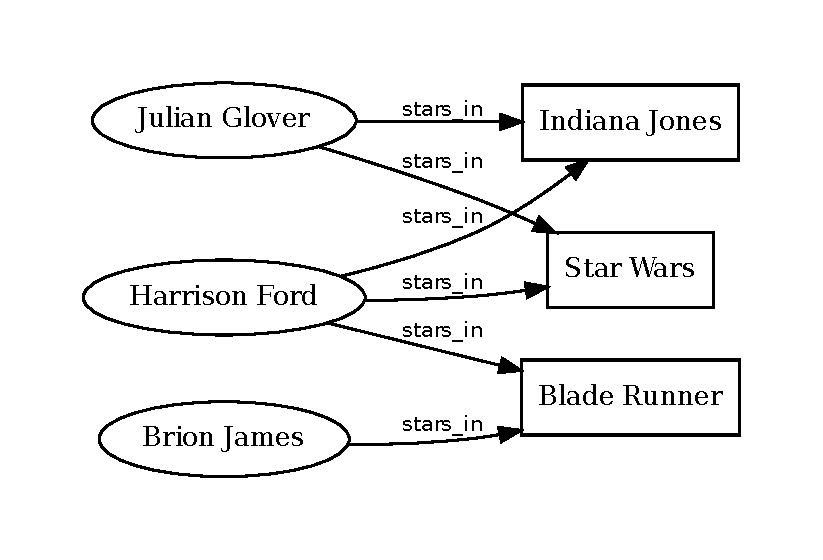
\includegraphics[width=0.45\textwidth]{graph}
\caption{Example input graph}
\label{fig:graph}
\end{figure}

\begin{figure}[h]
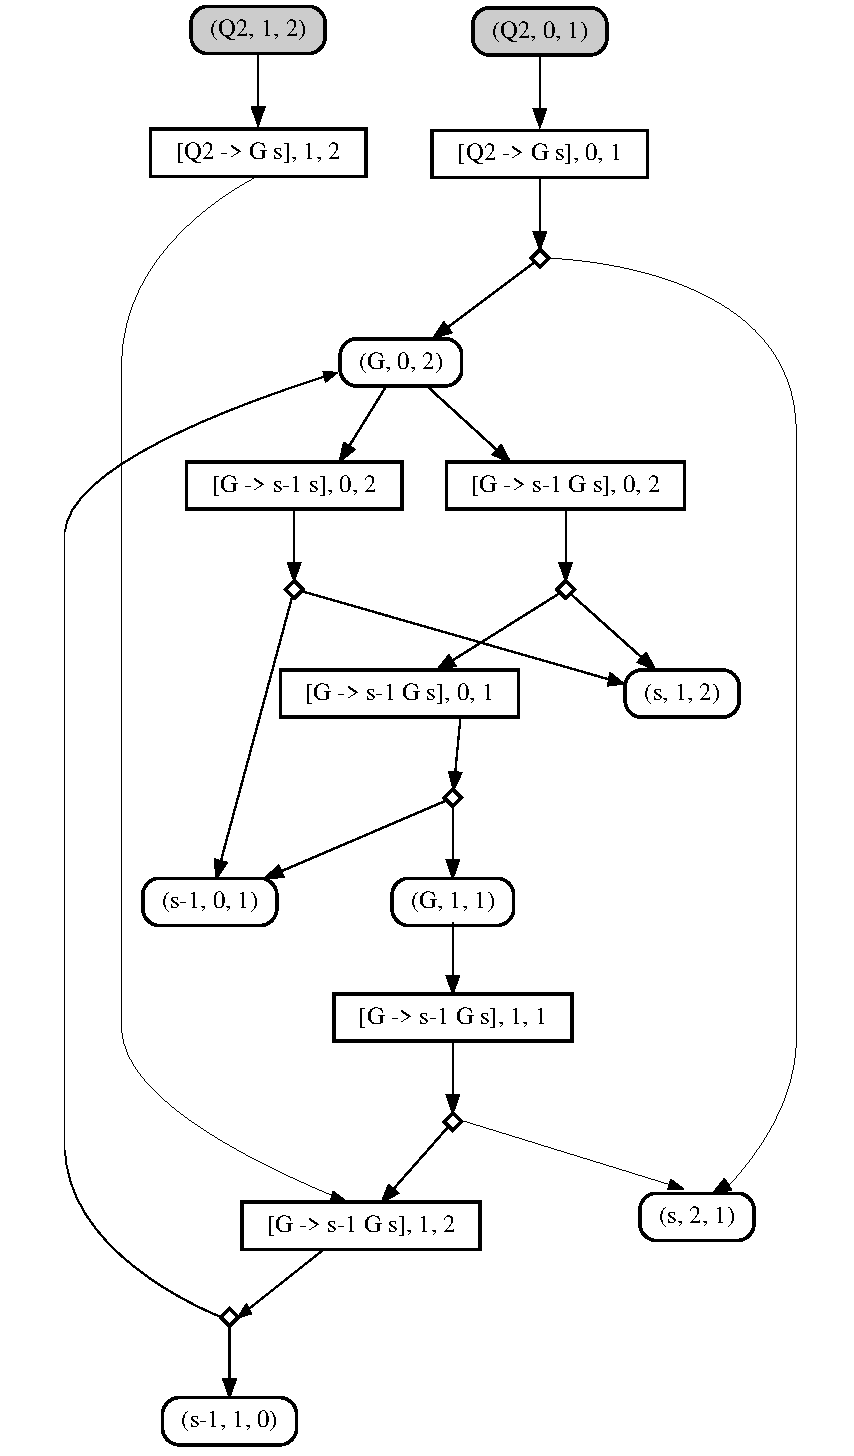
\includegraphics[scale=0.5]{sppf}
\caption{SPPF: result of applying the same generation Query 2 to the graph~\ref{fig:graph}}
\label{fig:sppf}
\end{figure}
